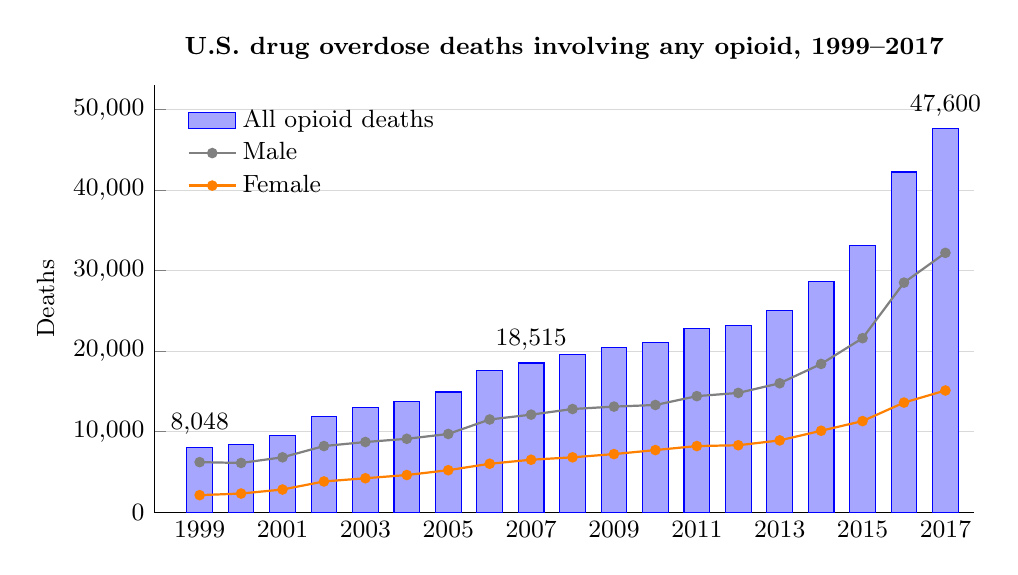
\begin{tikzpicture}
\begin{axis}[
  width=12cm, height=7cm,
  ymin=0, ymax=53000, clip=false, ytick={0,10000,...,50000},
  scaled y ticks=false,
  yticklabel style={/pgf/number format/1000 sep={\mathord{,}}},
  xmin=1997.9, xmax=2017.7, xtick={1999,2001,...,2017},
  xticklabel style={/pgf/number format/1000 sep={}},
  ymajorgrids, grid style={gray!30},
  axis lines*=left,
  tick label style={font=\small},
  ylabel={Deaths}, ylabel style={font=\small},
  title={U.S. drug overdose deaths involving any opioid, 1999--2017},
  title style={font=\small\bfseries},
  legend style={font=\small, draw=none, fill=none, at={(0.03,0.97)}, anchor=north west, legend columns=1},
  legend cell align=left
]
% total deaths involving any opioid (bars)
\addplot[ybar, bar width=0.62, draw=blue, fill=blue!35, area legend]
  coordinates {
  (1999,8048) (2000,8407) (2001,9496) (2002,11920) (2003,12940) (2004,13756)
  (2005,14918) (2006,17545) (2007,18515) (2008,19582) (2009,20422) (2010,21089)
  (2011,22784) (2012,23166) (2013,25052) (2014,28647) (2015,33091) (2016,42249)
  (2017,47600)};
\addlegendentry{All opioid deaths}
% male and female (read from the slide's chart, to the nearest 100)
\addplot[gray, thick, mark=*, mark size=1.5pt]
  coordinates {
  (1999,6200) (2000,6100) (2001,6800) (2002,8200) (2003,8700) (2004,9100)
  (2005,9700) (2006,11500) (2007,12100) (2008,12800) (2009,13100) (2010,13300)
  (2011,14400) (2012,14800) (2013,16000) (2014,18400) (2015,21600) (2016,28500)
  (2017,32200)};
\addlegendentry{Male}
\addplot[orange, thick, mark=*, mark size=1.5pt]
  coordinates {
  (1999,2100) (2000,2300) (2001,2800) (2002,3800) (2003,4200) (2004,4600)
  (2005,5200) (2006,6000) (2007,6500) (2008,6800) (2009,7200) (2010,7700)
  (2011,8200) (2012,8300) (2013,8900) (2014,10100) (2015,11300) (2016,13600)
  (2017,15100)};
\addlegendentry{Female}
\node[font=\small, above=1pt] at (axis cs:1999,8048) {8,048};
\node[font=\small, above=1pt] at (axis cs:2007,18515) {18,515};
\node[font=\small, above=1pt] at (axis cs:2017,47600) {47,600};
\end{axis}
\end{tikzpicture}
